\section{Specifications}
\subsection{Facebook Chatbot}
The service will be provided to the user by utilizing the Facebook chatbot. The following figure Fig. \ref{fig:facebook_overview} further details the general design of the system. Requests from the user will be processed by the bot using a text recognition software and our own database with information about various dishes.

\begin{figure}[htbp]
\centerline{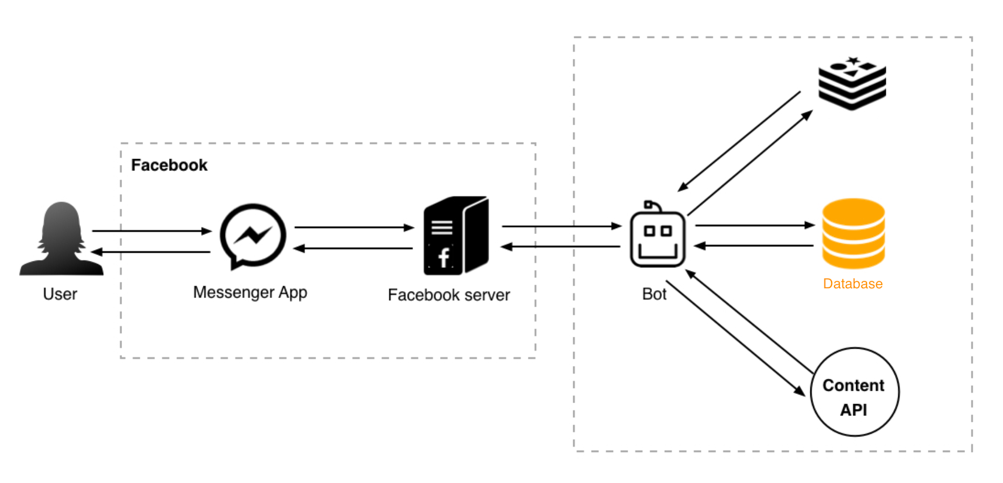
\includegraphics[width=\linewidth]{./pictures/facebook_overview}}
\caption{Overview of the system}
\label{fig:facebook_overview}
\end{figure}
\FloatBarrier

Using the Facebook Messenger as interface for our service, the user doesn't have to download a separate application and is already accustomed to navigate within the application and its usage. In order to use the service the user has to search for the \emph{Before Order} page on Facebook and send the profile a message by clicking the \emph{Send Message} button.

\begin{figure}[htbp]
\centerline{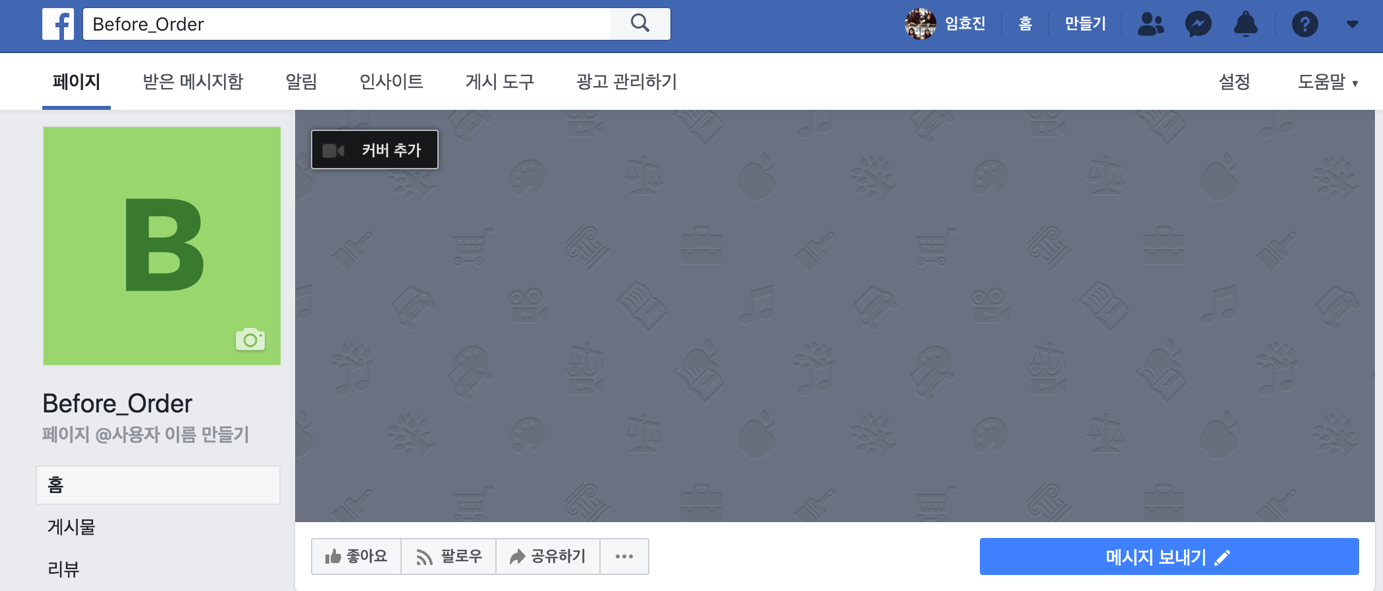
\includegraphics[width=\linewidth]{./pictures/facebook_profil}}
\caption{Chatbot profil on Facebook}
\label{fig:facebook_profil}
\end{figure}
\FloatBarrier

\subsubsection{Facebook messenger}

Given that the user has sent a message to the \emph{Before Order} service, the chat will be easily accessible from then on in the chatroom section of the Facebook Messenger application.

\begin{figure}[htbp]
\centerline{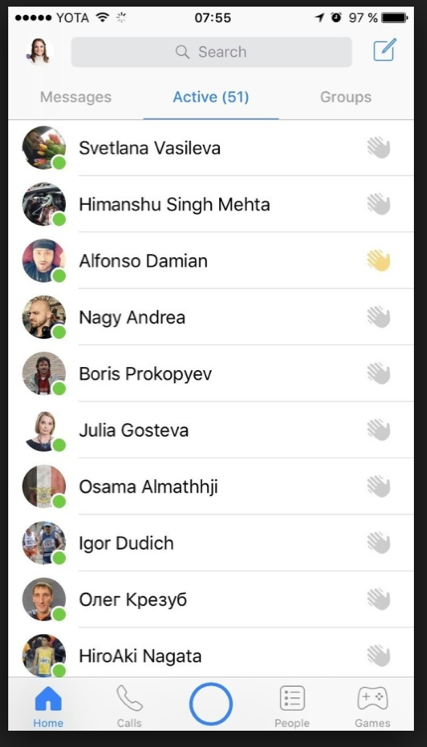
\includegraphics[height=\custompicheight]{./pictures/facebook_friends}}
\caption{Homescreen of the Facebook Messenger}
\label{fig:facebook_friends}
\end{figure}
\FloatBarrier

By selecting \emph{Before Order} from the list, the user is now able to provide a picture or dish names in the Korean alphabet to the chatbot by sending an image or a text message as shown in Fig. \ref{fig:facebook_message}

\begin{figure}[htbp]
\centerline{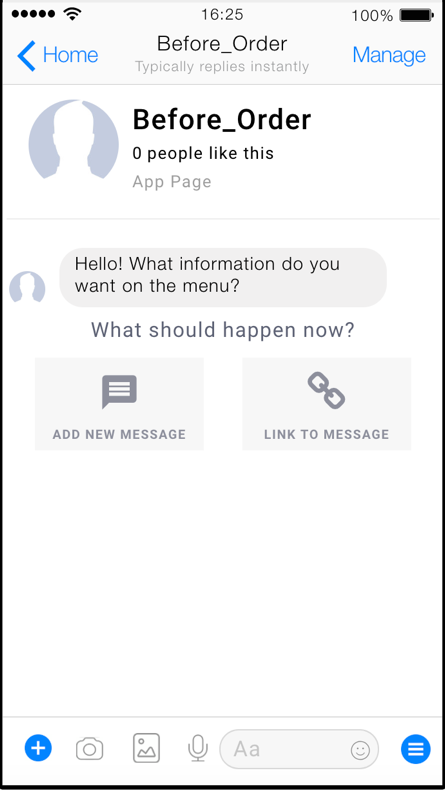
\includegraphics[height=\custompicheight]{./pictures/facebook_message}}
\caption{Chatroom with the \emph{Before Order} chatbot}
\label{fig:facebook_message}
\end{figure}
\FloatBarrier

\subsubsection{Chatbot input}

If the user sends the menu in form of a picture, the dish names have to be spelled out and need to be visible. The user can either send a picture that he took in the past or use the camera function in the Facebook Messenger to capture a picture and directly send it to the chatbot.

\begin{figure}[htbp]
\centerline{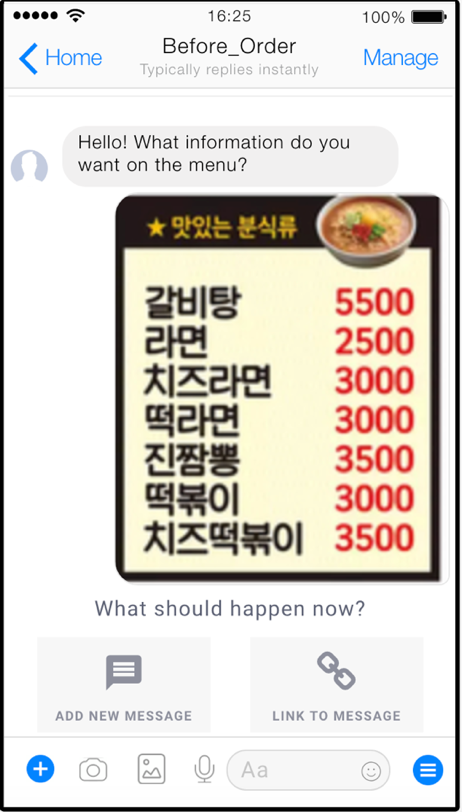
\includegraphics[height=\custompicheight]{./pictures/facebook_menu}}
\caption{Message to the chatbot including a picture of a menu}
\label{fig:facebook_menu}
\end{figure}
\FloatBarrier

Using a text recognition API and analyzing the image we are able to provide a list with all the found and supported dish names. The user is now able to select a dish that he wants more detailed information about as shown in Fig. \ref{fig:facebook_response}.

\begin{figure}[htbp]
\centerline{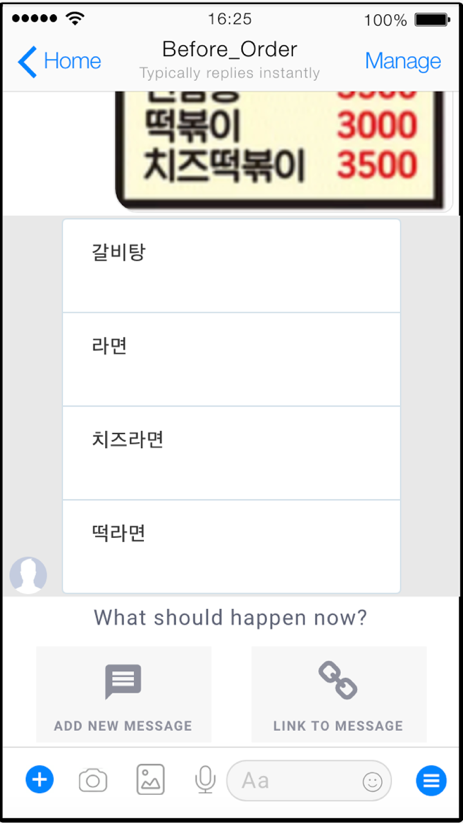
\includegraphics[height=\custompicheight]{./pictures/facebook_response}}
\caption{Response of the chatbot with all the found dishes}
\label{fig:facebook_response}
\end{figure}
\FloatBarrier

\begin{figure}[htbp]
\centerline{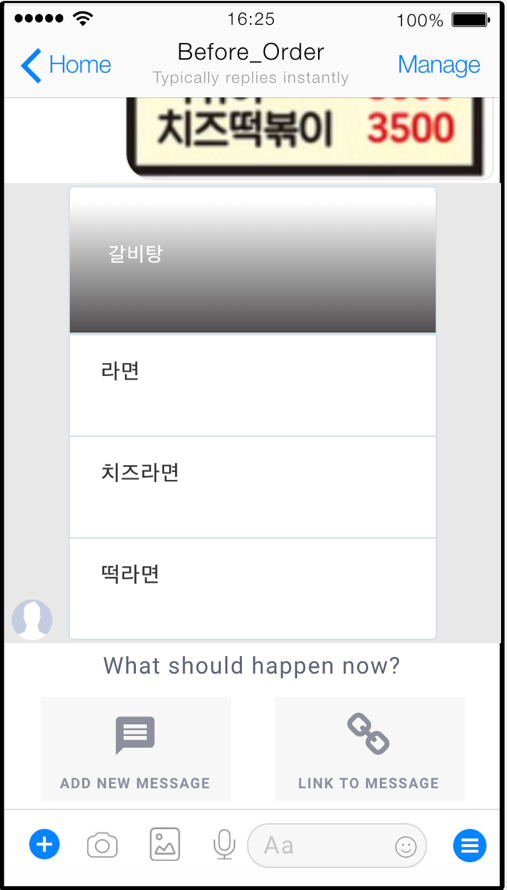
\includegraphics[height=\custompicheight]{./pictures/facebook_response_selection}}
\caption{User selecting a dish from the list}
\label{fig:facebook_response_selection}
\end{figure}
\FloatBarrier

\subsubsection{Processing of the input}

\begin{itemize}
\item Get the information from database

The information for dishes will be provided by our own database. Instead of using an open-source API for translating Korean words to English we will be using an own mapping between English and Korean dish names as the common translators don't support uncommon dish names or variants of dish names. Therefore each dish will have an English and an Korean name associated with it to make it possible to search for dishes inside the database using Korean letters. Hence most of the processes in and around the database will have to support and communicate using the UTF-8 encoding. The database will also contain a one or two sentence description for each dish, a list with its main ingredients and additional flags, such as \emph{spicy}. Managing and searching for information in this kind of database has the advantage, that:

\begin{itemize}
\item information for every dish is consistent and unlike as in popular search machines, such as \emph{Wikipedia} and \emph{Google}, every entry in the database will have the common information
\item we can be sure information and names in the database refers to a dish, which enables us to filter out random text sequences and unrelated Korean words and sentences
\item we don't have to rely on the authenticity of information from a third party
\end{itemize}

\item Server that can run chatbot and chatbot service

We will use Azure Virtual Server to run our chatbot. There are three parts in our chatbot service in the virtual machine. First one is a script that is connected with Facebook Chatbot API. This script will have scenarios to answer users' requests and call other scripts to provide information to the users. Second one is to recognize the texts from a picture that users send using Computer Vision API, and the last one is for interacting with the database. When the chatbot gets the input from the users, it will call the script for text recognition. The results will be double-checked with the database to ensure only supported dishes are sent to the user in form of a list. By selecting a dish from the list the user sends another request to the chatbot. The chatbot will then call the script for retrieving data from the database and return the detailed information about the dish to the user.

\item Vision api connection

When chatbot calls the script that is connected with Computer Vision API, it will send the picture to the Computer Vision API and get the results from it in a json format. It includes a request using the key and endpoint of the Computer Vision API. The script also includes a refinement part, where it refines the result text and formats the result of the text recognition as a list. The list will then be returned to the chatbot.
\end{itemize}
\FloatBarrier

\subsubsection{Chatbot output}

\begin{figure}[htbp]
\centerline{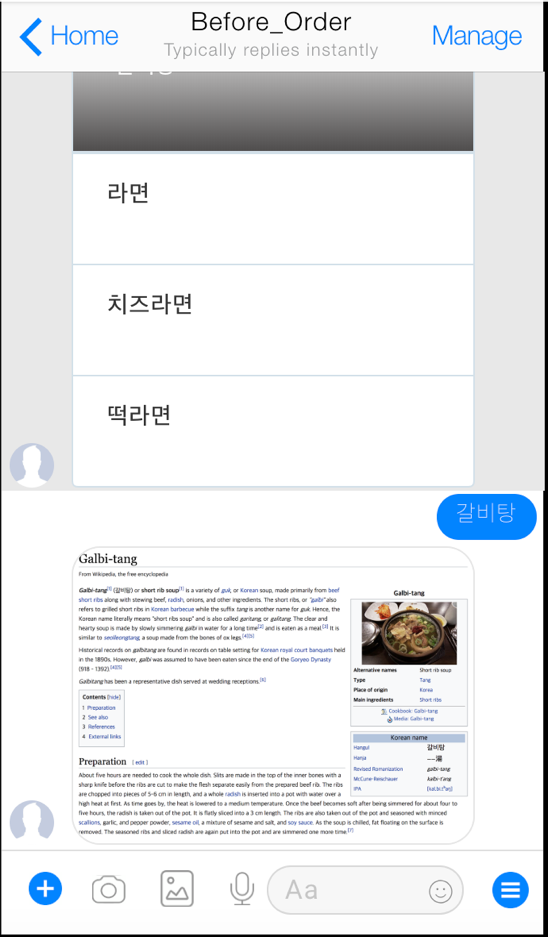
\includegraphics[height=\custompicheight]{./pictures/facebook_dish_information}}
\caption{Detailed informations about the selected dish}
\label{fig:facebook_dish_information}
\end{figure}
\FloatBarrier

Although we can not represent it in this prototype, we plan to provide information from our internal database. Users will be able to receive images of the dishes and a detailed description with ingredients...

\subsubsection{Exit}
If you need information about other menus, please feel free to send us a message.